%% Tasks for Proposed Solution

The work for the proposed solution will be broken down into three phases.  The first phase will involve the actual implementation of the daemon and benchmarking the stock random number generator with the DIEHARD and NIST standards.  Two people will work on the daemon while the other two work on benchmarking and post processing.  The second phase will involve collecting data and testing the solution.  Because the Dragonboard is a development platform and is not intended to be carried on a person, data will need to be collected from accelerometers on production mobile devices.  This data will be compared with the Dragonboard to determine the increase in entropy from moving the acceleromter more.  During this phase, the implemented solution will be benchmarked with DIEHARD and NIST for comparision to the stock random number generator.  Two people will collect the accelerometer data while the third and fourth benchmark and measure power usage of the solution.  The final phase of the project will be to prepare the report.  Major sections of the report can be worked on independently, in parallel.  The group will meet to discuss and finalize the conclusion section and submit the report.  

All of the tasks are laid out on the Ghantt chart shown

\begin{figure*}[t]
	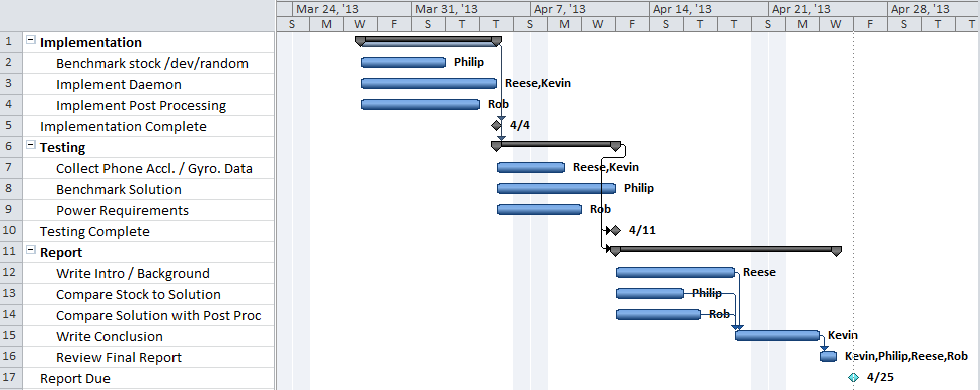
\includegraphics[width=\columnwidth]{proj-ghantt-v3}
	\caption{Assigned tasks and estimated time of completion}
	\label{Ghantt Chart}
\end{figure*}